\chapter{Fully-Hadronic: EFT Benchmark study}
\label{sec:FHEFTBenchmarkDNN}
% Main 12 Benchmark citation: \cite{Carvalho:2015ttv}
% another 7 Benchmark citation: \cite{Capozi:2019xsi}

For the fully-hadronic channel, parametric DNN approach was tested. For this, the the parametric DNN training,
we considered the similar approach as utilized for the SM fully-hadronic DNN, i.e., train the two DNN network.
First DNN network acts as $bb\gamma\gamma$ killer and another for the separation of signal w.r.t. other backgrounds.

The details of two DNN network as follows:
\begin{itemize}
  \item \textbf{bb$\gamma\gamma$ killer}: Trained for reducing the overlap of WW$\gamma\gamma$ and bb$\gamma\gamma$. For this training, all twenty nodes of bb$\gamma\gamma$ is considered signal,
  and in addition to the backgrounds in (Tab.~\ref{tab:fullyHadronicMCBkg_Appendix}), all 20 nodes of WW$\gamma\gamma$ is included as an additional background.
  \item \textbf{WW$\gamma\gamma$ identifier}: Trained for the separation of signal ($HH \rightarrow WW\gamma\gamma$, included all 20 nodes as singal) and backgrounds (as listed in Tab.~\ref{tab:fullyHadronicMCBkg_Appendix}).
\end{itemize}

\begin{table}[!htbp]
  \begin{center}
          \begin{tabular}{|c|}
                \hline
                \textbf{MC Samples}  \\ \hline
                DiPhoJetsBox\_MGG-80toInf  \\ \hline
                GJet\_40toInf $\Rightarrow$ Data-Driven QCD \\ \hline
                HT-binned QCD  $\Rightarrow$ Data-Driven QCD\\ \hline
                tt$\gamma\gamma+$0Jets  \\ \hline
                tt$\gamma+$Jets  \\ \hline
                % ttH  \\ \hline
                % VH   \\ \hline
                % VBF-H    \\ \hline
                % GluGluH \\ \hline
          \end{tabular}
  \caption{MC list for Fully-Hadronic}
  \label{tab:fullyHadronicMCBkg_Appendix}
  \end{center}
\end{table}

The list of input variables and DNN model architecture remains same as
Tab.~\ref{tab:FHDNNinputfeatures1} and Fig.~\ref{fig:FH_DNN_Architecture}.

\clearpage
\section{\texorpdfstring{bb$\gamma\gamma$}{bbyy} killer: DNN details}

\begin{figure}[!htbp]
    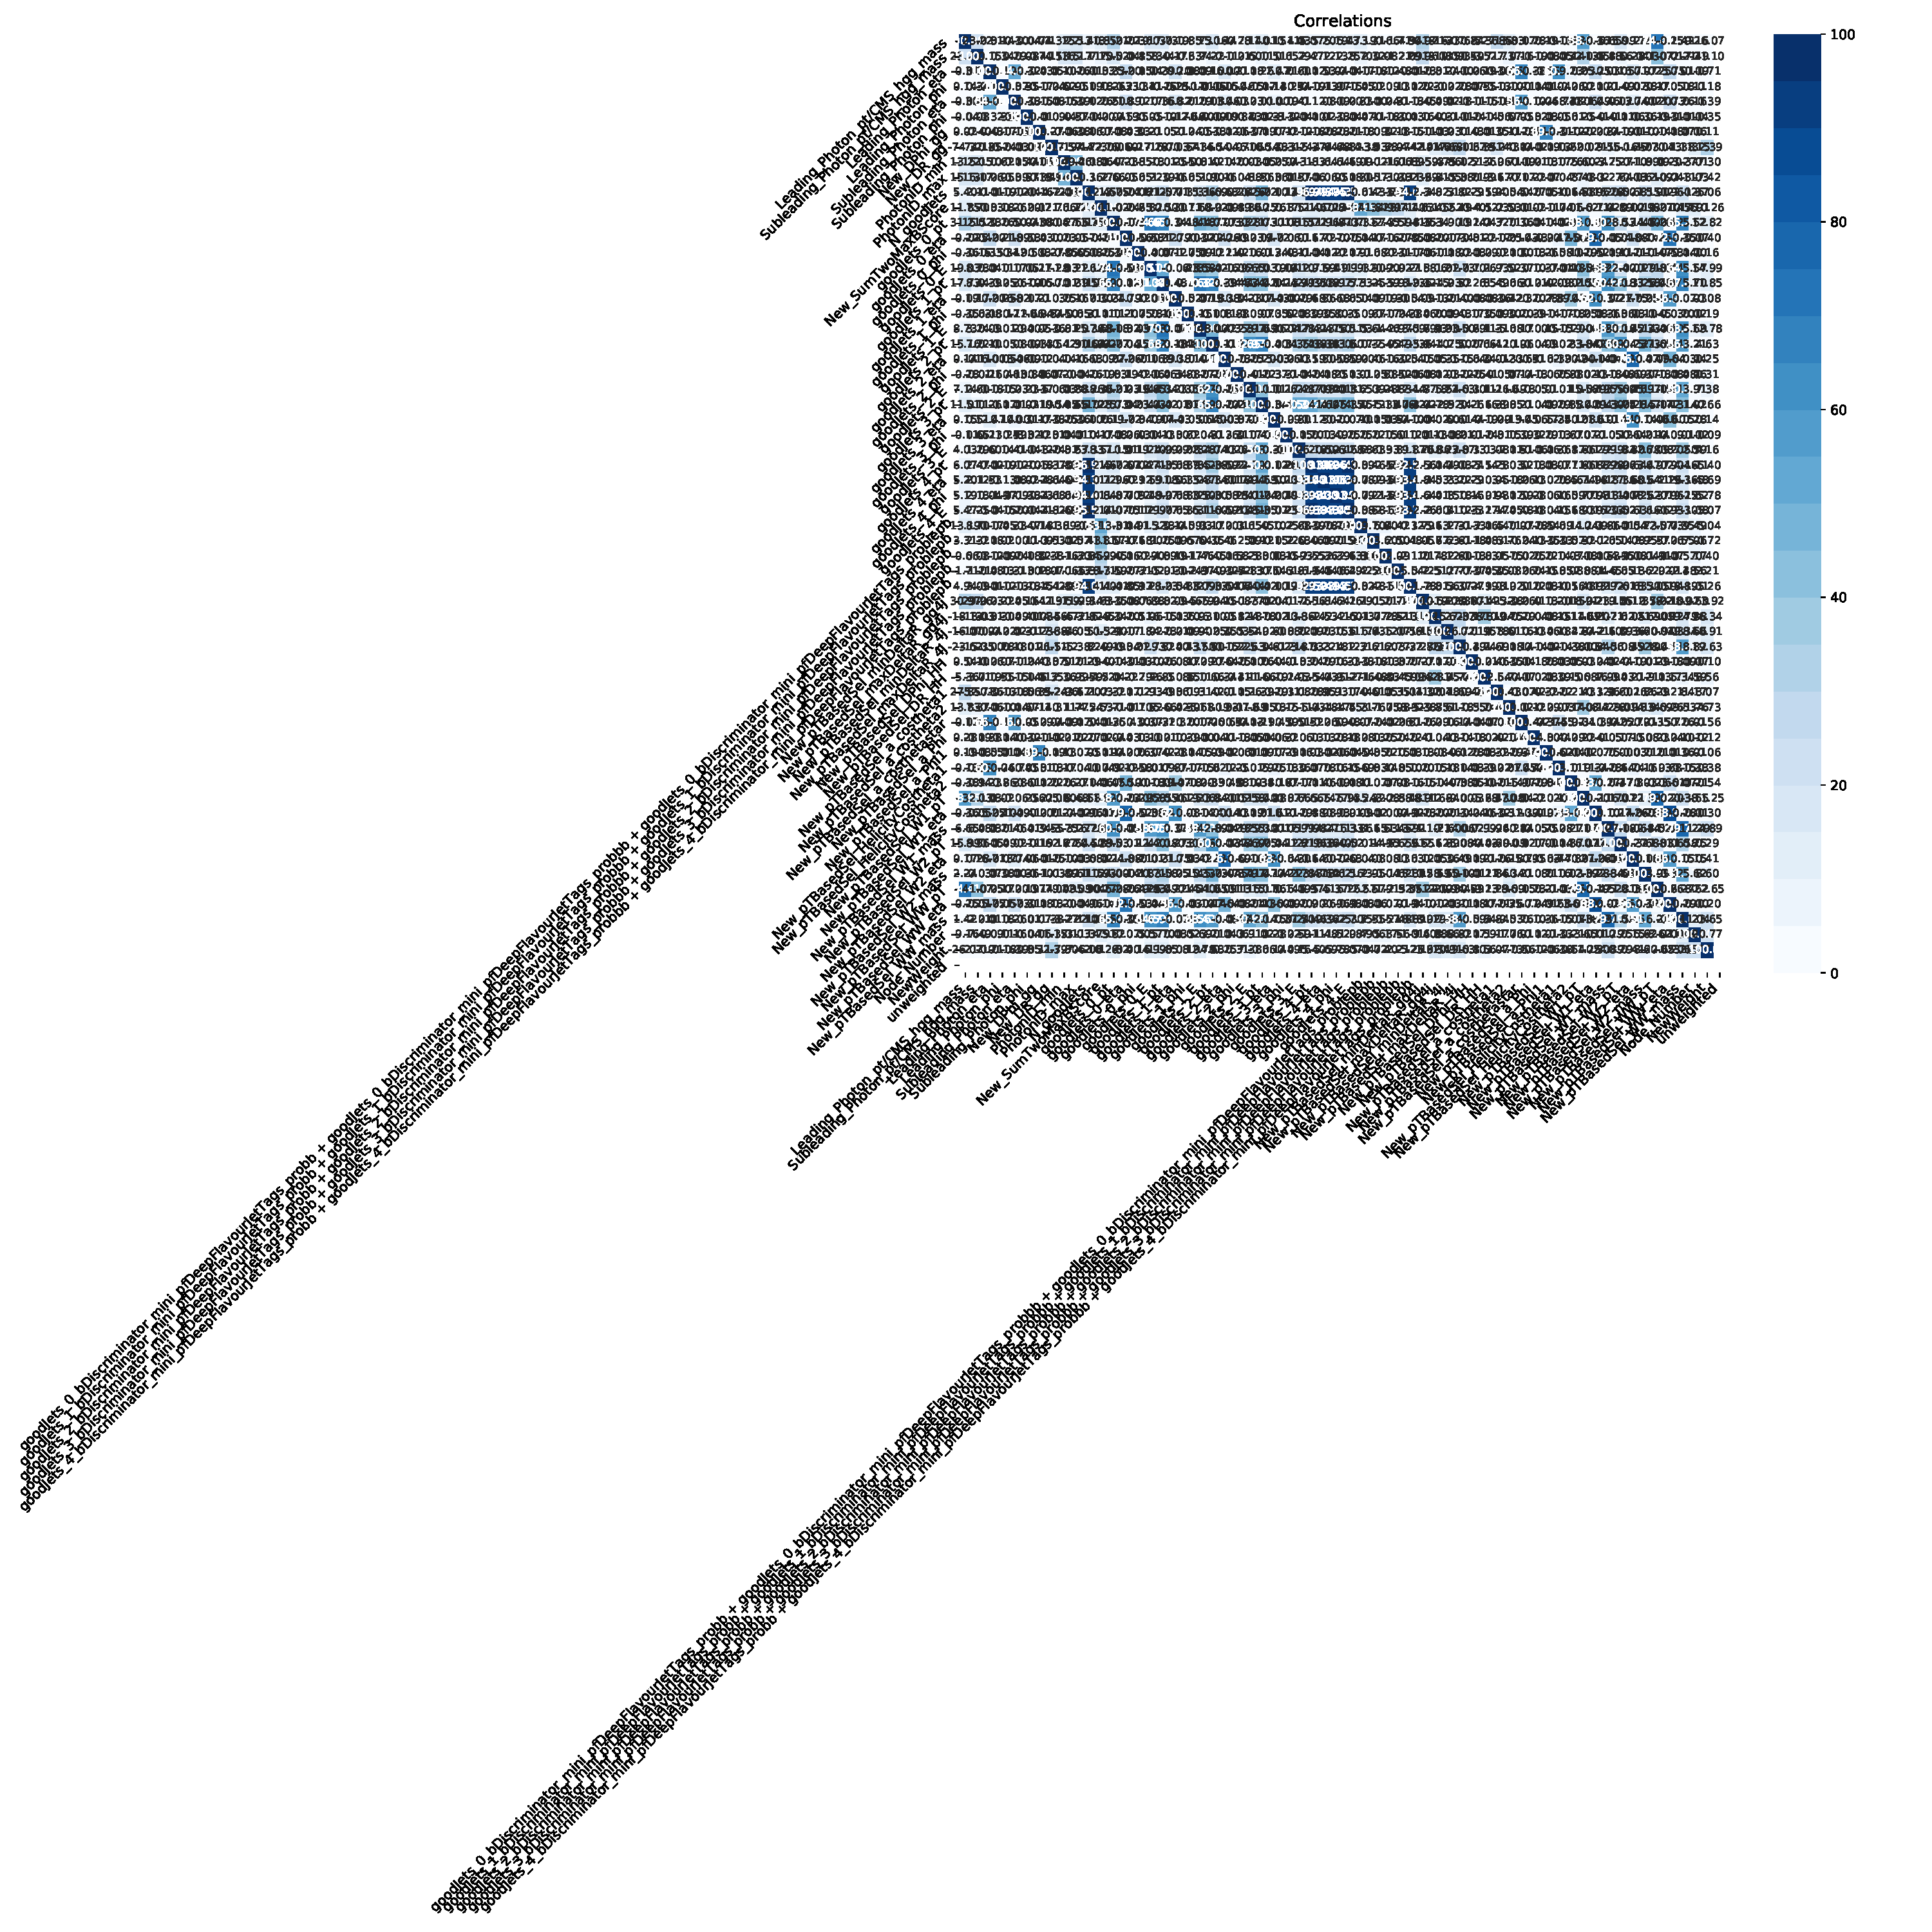
\includegraphics[width=\textwidth,trim={17cm 17cm 0 0},clip=true]{Sections/HHWWgg/images/FH_DNN/EFT/HHWWyyDNN_binary_BBggAsSignal_E500_B250_BalanceYields/correlation_plot.pdf}
    \caption{Correlation of Fully-Hadronic DNN bb$\gamma \gamma$ killer training input features}
    \label{fig:FH_DNN_CorrelationPlot_bbgg}
\end{figure}

\begin{figure}[!htbp]
    \centering
    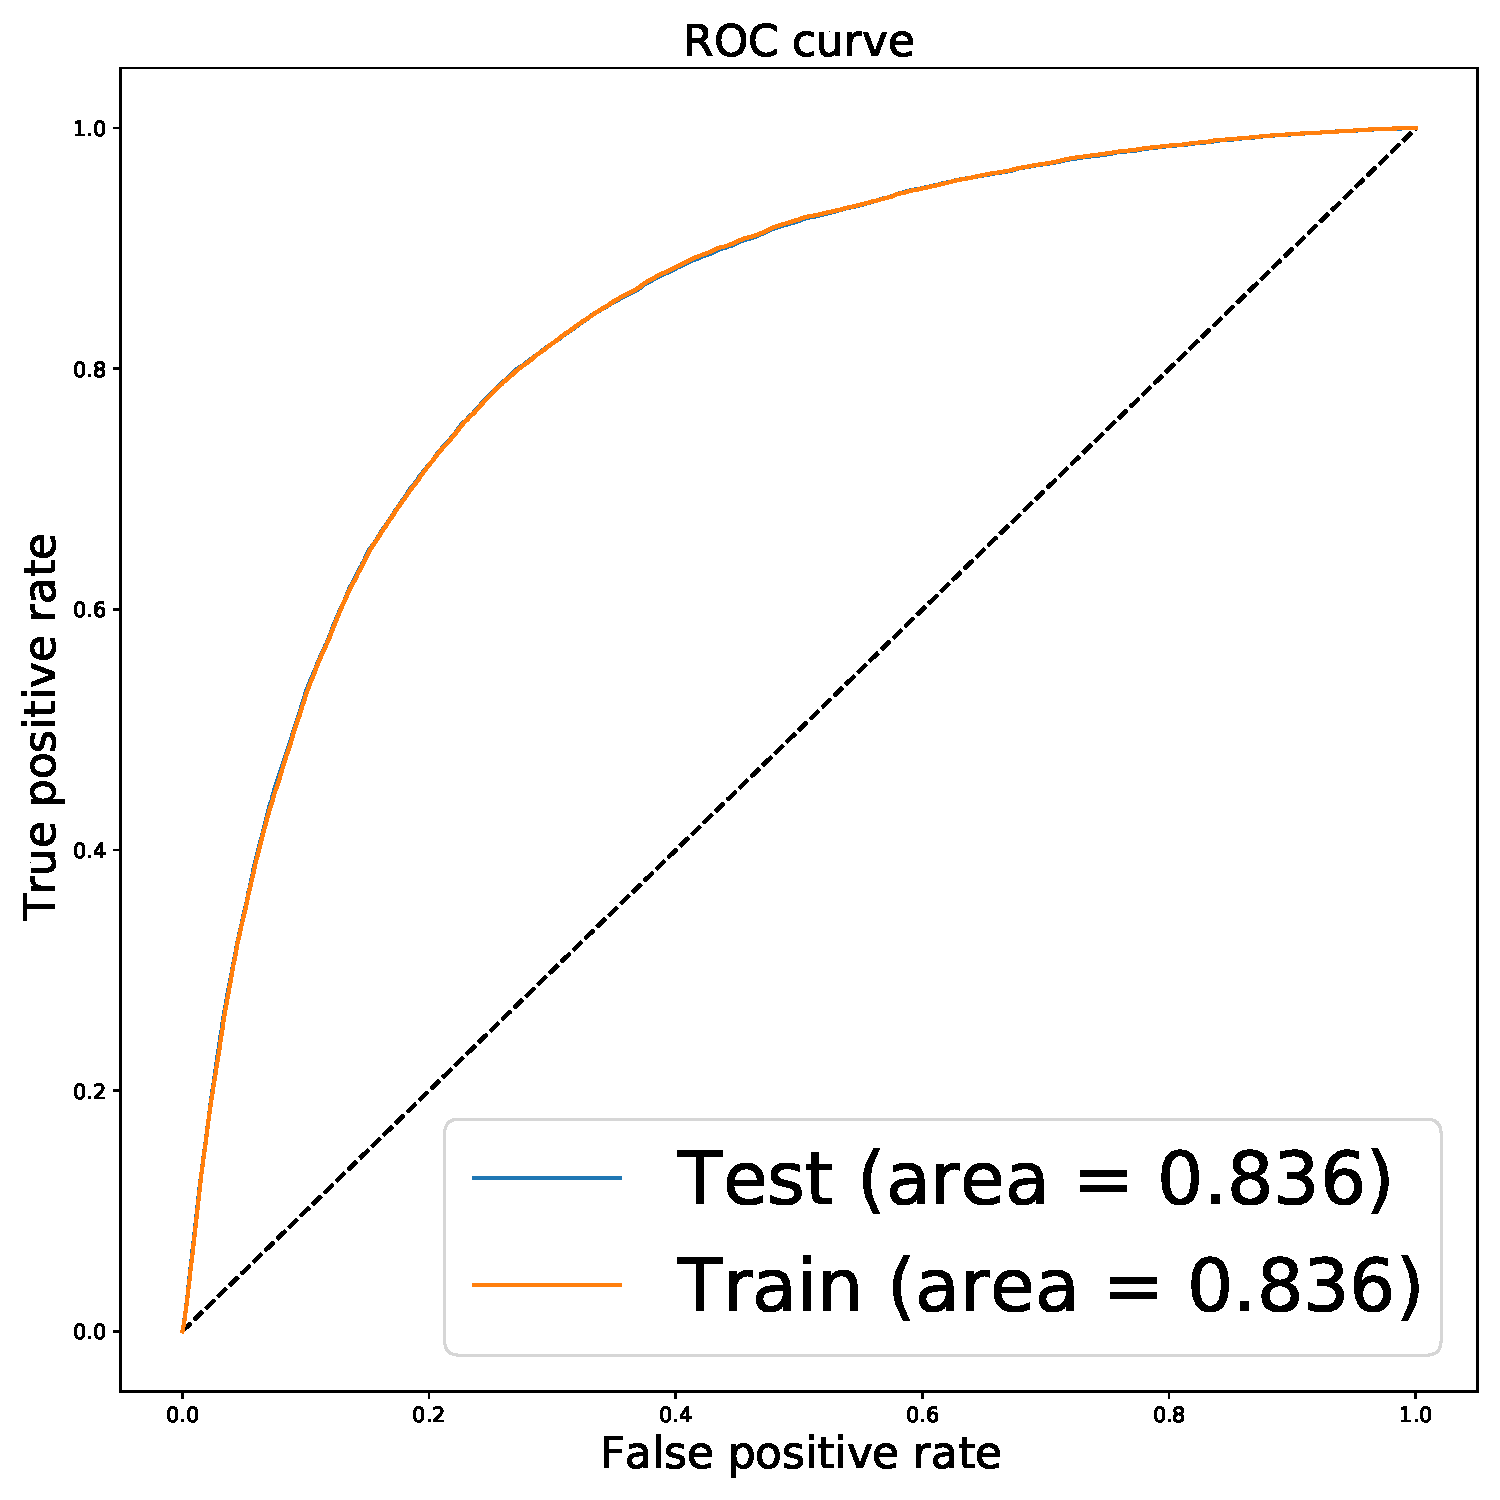
\includegraphics[scale=0.4]{Sections/HHWWgg/images/FH_DNN/EFT/HHWWyyDNN_binary_BBggAsSignal_E500_B250_BalanceYields/ROC.pdf}%
    \caption{ROC curve for bb$\gamma \gamma$ killer Fully-Hadronic DNN}
    \label{fig:FH_DNN_ROC_bbgg}
\end{figure}

\begin{figure}[!htbp]
\centering
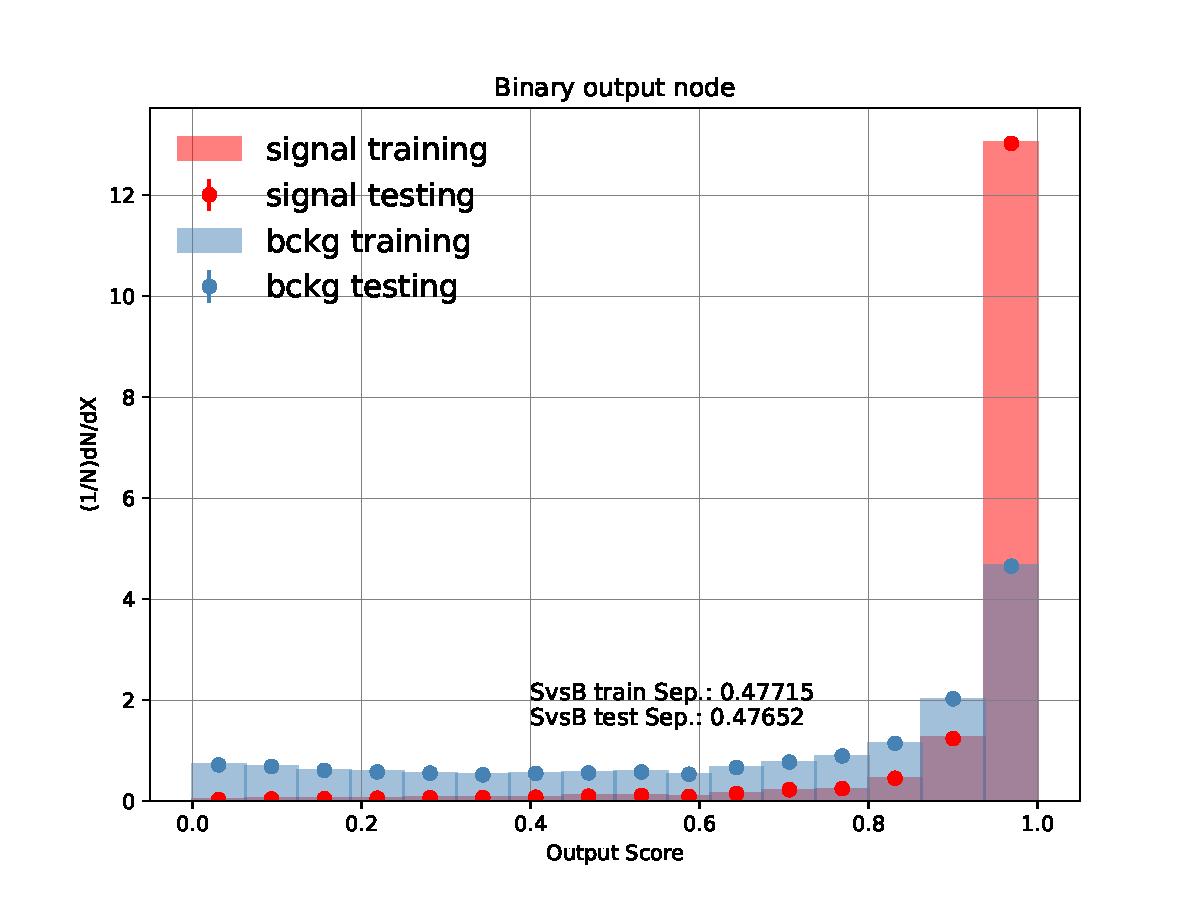
\includegraphics[scale=0.6]{Sections/HHWWgg/images/FH_DNN/EFT/HHWWyyDNN_binary_BBggAsSignal_E500_B250_BalanceYields/overfitting_plot_BinaryClassifier_Binary.pdf}%
\caption{Output score of Fully-Hadronic DNN bb$\gamma \gamma$ killer training}
\label{fig:FH_DNN_OutputScore_bbgg}
\end{figure}

\clearpage
\section{\texorpdfstring{WW$\gamma\gamma$}{WWyy} identifier: DNN details}

\begin{figure}[!htbp]
    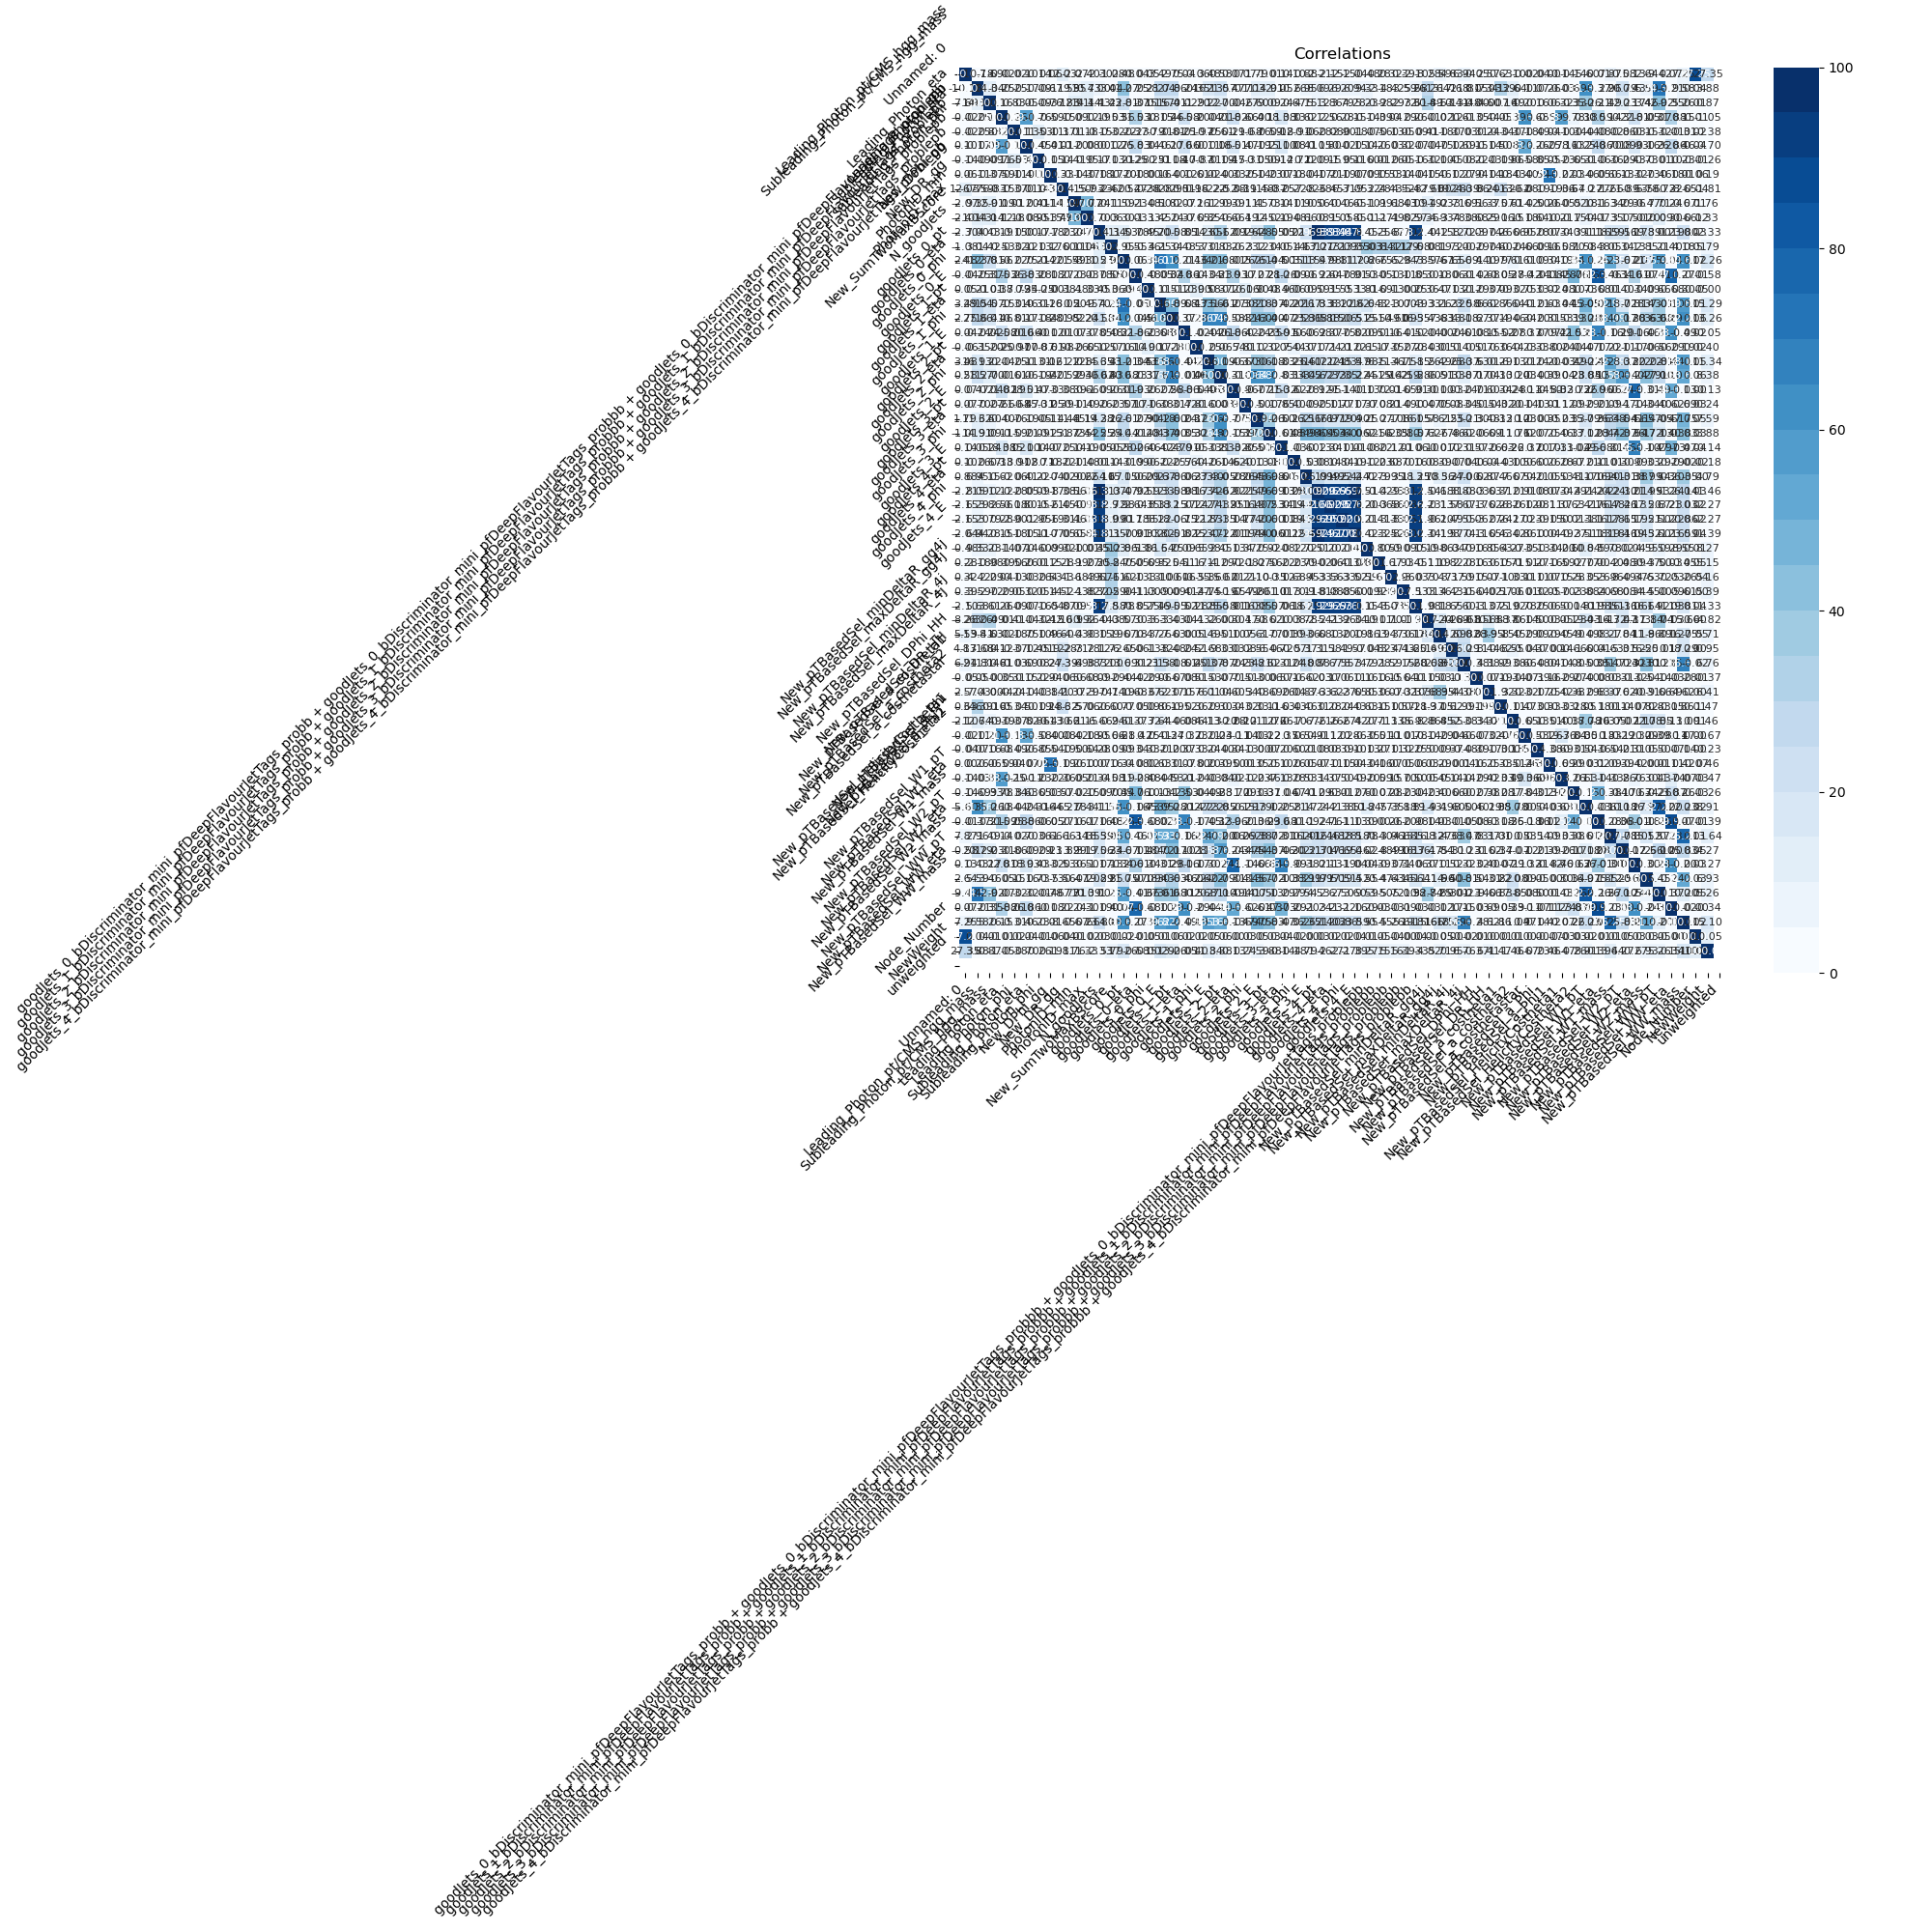
\includegraphics[width=\textwidth,trim={17cm 17cm 0 0},clip=true]{Sections/HHWWgg/images/FH_DNN/EFT/HHWWyyDNN_binary_scan_BalanceYields/correlation_plot.png}
    \caption{Correlation of Fully-Hadronic DNN WW$\gamma \gamma$ identifier training input features}
    \label{fig:FH_DNN_CorrelationPlot_appendix}
\end{figure}

\begin{figure}[!htbp]
    \centering
    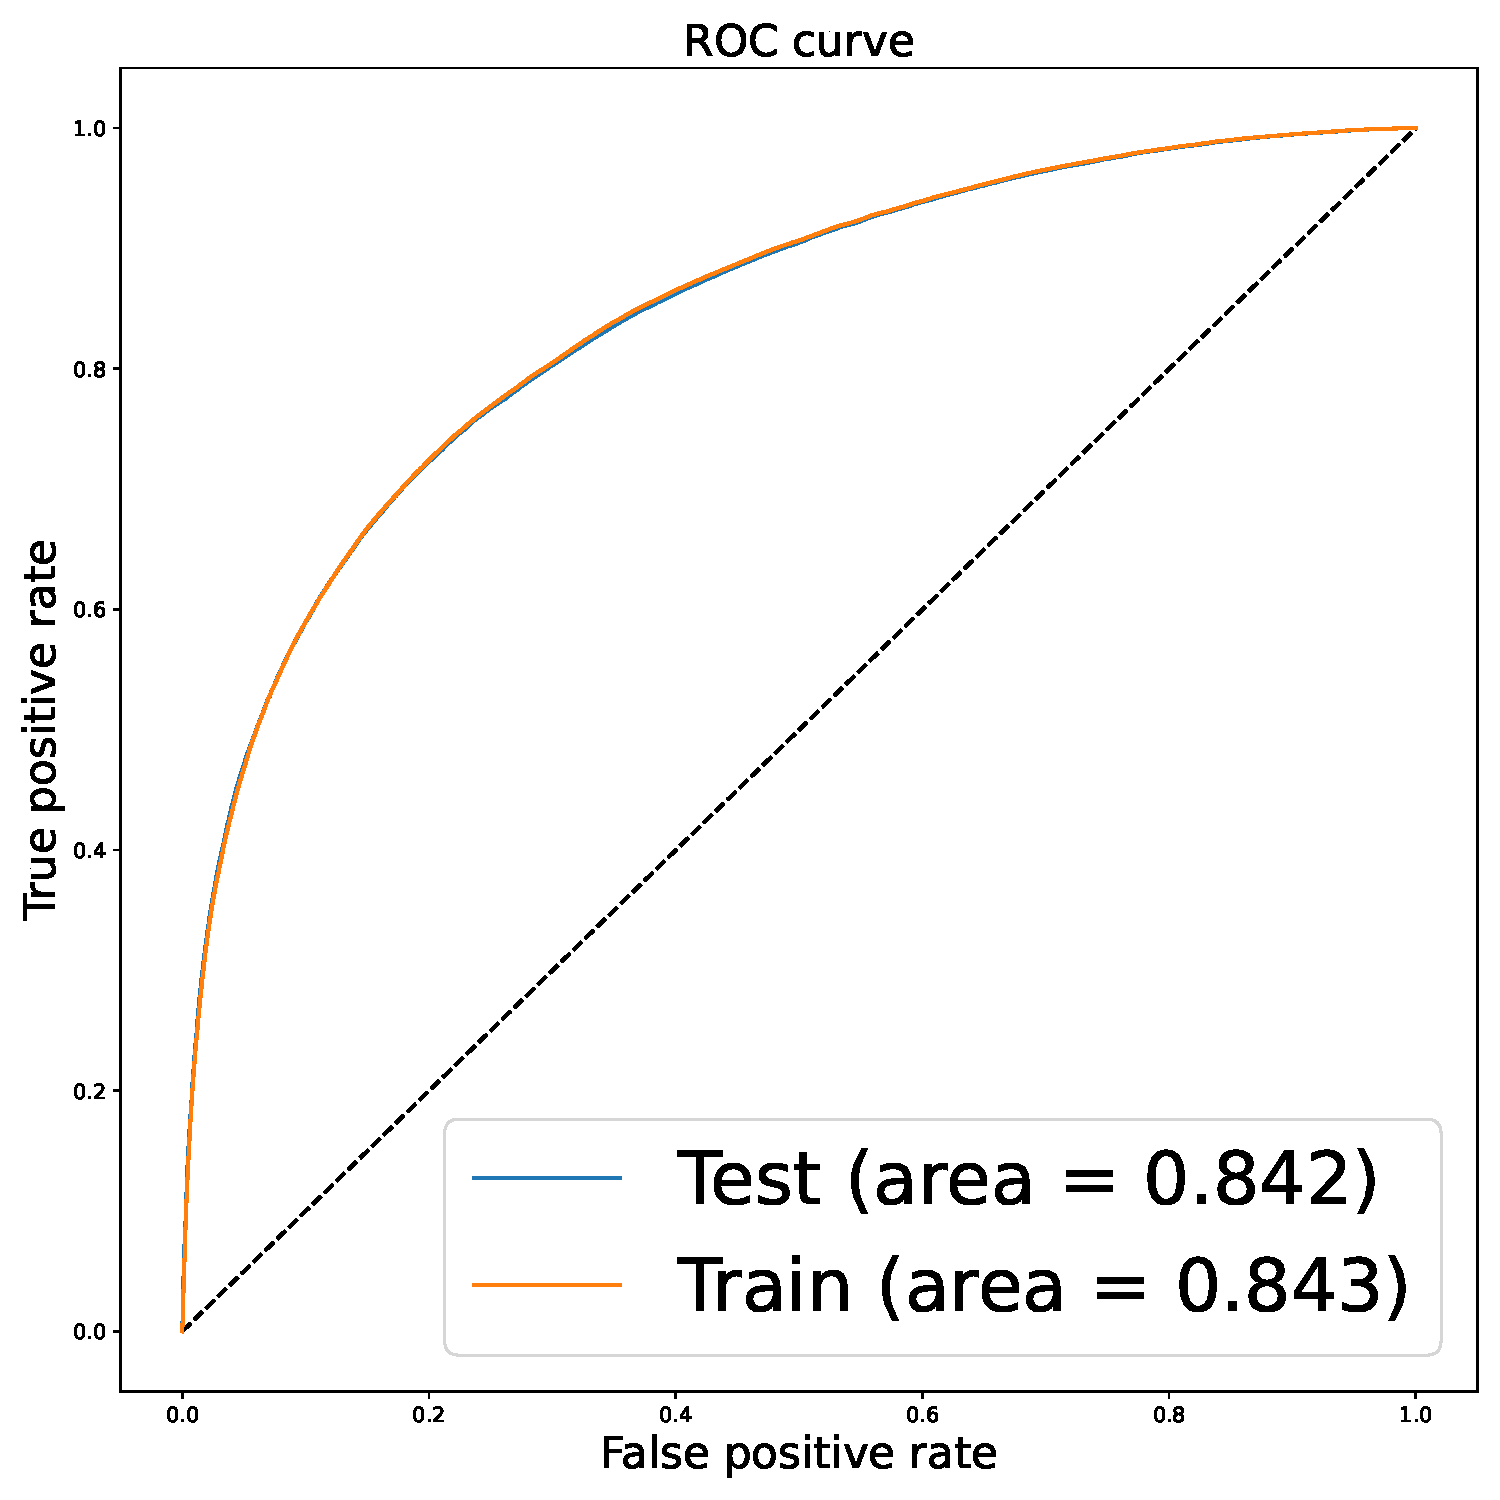
\includegraphics[scale=0.4]{Sections/HHWWgg/images/FH_DNN/EFT/HHWWyyDNN_binary_scan_BalanceYields/ROC.pdf}%
    \caption{ROC curve for WW$\gamma \gamma$ identifier Fully-Hadronic DNN}
    \label{fig:FH_DNN_ROC_appendix}
\end{figure}

\begin{figure}[!htbp]
\centering
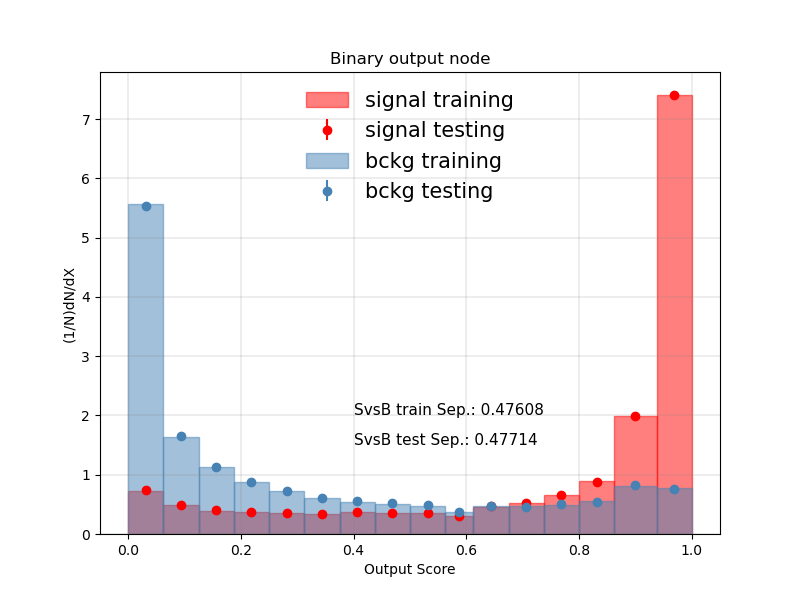
\includegraphics[scale=0.6]{Sections/HHWWgg/images/FH_DNN/EFT/HHWWyyDNN_binary_scan_BalanceYields/overfitting_plot_BinaryClassifier_Binary.png}%
\caption{Output score of Fully-Hadronic DNN WW$\gamma \gamma$ identifier training}
\label{fig:FH_DNN_OutputScore_appendix}
\end{figure}
